%!TEX root = ../main.tex

\chapter{Justificación económica}\label{cap:economica}

\section{Introducción}

En este capítulo se aborda el análisis económico y financiero del ``Sistema inteligente de recomendación para la gestión del cuidado de personas con discapacidad en Argentina''. El propósito central es detallar los recursos monetarios que exige la propuesta, definir las estrategias necesarias para garantizar su sostenibilidad una vez concluida la fase universitaria y determinar las condiciones bajo las cuales el proyecto resulta económicamente viable.

Para lograr una estimación certera, la evaluación distingue claramente entre el desarrollo del prototipo académico y su eventual implementación en un entorno de producción real. Durante la etapa del prototipo, no se asigna un valor monetario a las horas de trabajo dedicadas a la investigación, el diseño de software, la programación ni al trabajo de campo. Al tratarse de actividades enmarcadas en el ámbito académico, representan un esfuerzo técnico e intelectual que no implica un desembolso directo para el proyecto. En consecuencia, la inversión considerada en esta fase inicial se limita exclusivamente a los gastos monetarios imprescindibles para contratar los servicios digitales y la infraestructura tecnológica que hacen posible el funcionamiento del sistema.

\section{Metodología y alcance}

La factibilidad del proyecto se analiza mediante un flujo de fondos proyectado a cinco años y expresado en dólares estadounidenses. Para evaluar la rentabilidad financiera de la propuesta, se utilizan como indicadores clave el flujo de fondos, el período de repago, el período de repago descontado, el Valor Actual Neto (VAN) y la Tasa Interna de Retorno (TIR). Adicionalmente, se incorpora el cálculo del punto de equilibrio, el cual funciona como una referencia para identificar el nivel mínimo de ingresos que el sistema debe generar para cubrir sus costos operativos.

La decisión de estructurar la evaluación en dólares responde a que los principales servicios tecnológicos e infraestructura en la nube cotizan habitualmente en esta moneda.

\section{Análisis de mercado y competidores}

\subsection{Tamaño del mercado}

Según el INDEC, el 10,2~\% de la población de 6 años y más que vive en localidades urbanas tiene alguna discapacidad \citep{indec2018}. El Registro Nacional de Personas con Discapacidad contabilizaba, a noviembre de 2023, 1.680.723 personas con el Certificado Único de Discapacidad vigente \citep{andis2023}. Esta cifra se toma como una cota inferior del mercado potencial, porque cada persona certificada suele tener al menos una persona que la cuida, y porque no incluye a quienes no tramitaron el certificado.

El mercado se divide en tres segmentos. El primero son las personas que cuidan solas a un familiar, que usan el plan gratuito. El segundo son las familias que reparten el cuidado entre varias personas o contrataron a un cuidador, a las que se dirige el plan Intermedio. El tercero son las clínicas, residencias y centros de día, que necesitan supervisar el trabajo de varios empleados y contratan el plan Plus. El modelo de negocio es, por lo tanto, B2C para las familias y B2B para las instituciones, con una base gratuita.

La meta del escenario base es conservadora. Al quinto año proyecta 205 suscripciones pagas, lo que equivale a alrededor del 0,012~\% de las personas con certificado vigente.

\subsection{Competidores y precios de referencia}

\begin{table}[H]
\centering
\caption{Competidores y precios de referencia}\label{tab:c5-competidores}
\small
\begin{tabularx}{\textwidth}{l >{\raggedright\arraybackslash}X >{\raggedright\arraybackslash}X}
\toprule
\tb{Producto} & \tb{Modelo y precio} & \tb{Diferencia con la propuesta} \\
\midrule
CaringBridge & Gratuito, sostenido por donaciones \citep{caringbridge} & Comunicación con la red de apoyo, sin gestión del cuidado ni orientación \\
Lotsa Helping Hands & Gratuito \citep{lotsa} & Coordinación de tareas, sin registro por persona ni orientación \\
Medisafe & Suscripción de USD 4,99 por mes o USD 39,99 por año fuera de Estados Unidos desde 2026 \citep{medisafe2026} & Solo adherencia a la medicación \\
Acompañar & Plan Básico gratis con lo esencial, Intermedio USD 5 y Plus USD 15 por mes & Integra organización, grupo, trámites del contexto argentino y recomendaciones explicadas \\
\bottomrule
\end{tabularx}
\end{table}

El precio del plan Intermedio se ubica en el mismo nivel que la suscripción de Medisafe, que resuelve solo una parte del cuidado, y los productos gratuitos no cubren la gestión ni la orientación. Esto respalda la decisión de mantener gratis lo esencial y cobrar por la coordinación del grupo y la orientación.

\section{Modelo de ingresos propuesto}

La plataforma adopta un modelo de suscripción con una base gratuita y dos planes pagos. Lo básico del día a día, la línea del día, la medicación, el calendario, los documentos y la emergencia, es gratis siempre, y la emergencia nunca se cobra. Los planes pagos suman la guía de trámites, el diario, los recursos recomendados y la posibilidad de sumar cuidadores y observadores al grupo, cada uno con su propia cuenta.

Quien paga es el dueño del grupo, ya sea una familia o una institución. Las clínicas, residencias y centros de día contratan el plan Plus, que no tiene límite de pacientes ni de empleados e incluye el panel para supervisar lo que registra cada uno. Los cuidadores que forman parte de un grupo no pagan nada, porque los cubre el plan de su dueño.

\begin{table}[H]
\centering
\caption{Planes de la plataforma}\label{tab:c5-1}
\small
\begin{tabularx}{\textwidth}{l l >{\raggedright\arraybackslash}X}
\toprule
\tb{Plan} & \tb{Precio} & \tb{Qué incluye} \\
\midrule
Básico & USD 0 (gratis) & Una persona a cargo, cuidada por quien tiene la cuenta. Tu día, medicación, calendario, documentos (100 MB) y emergencia. \\
Intermedio & USD 5 por mes & Hasta cinco personas a cargo y tres integrantes en el grupo. Suma guía de trámites, diario con resumen del último mes, recursos recomendados, tu bienestar y documentos (1 GB). \\
Plus & USD 15 por mes & Personas e integrantes sin límite, artículos de especialistas, cumplimiento de cada cuidador, historial de un año y documentos (10 GB). Es el plan de las clínicas y residencias. \\
\bottomrule
\end{tabularx}
\end{table}

Para la proyección se contempla una adopción gradual de suscripciones pagas. Las cantidades corresponden a promedios anuales y no incluyen las cuentas gratuitas, que no generan ingresos. En el plan Plus se cuentan tanto familias que coordinan a muchas personas como instituciones.

\begin{table}[H]
\centering
\caption{Proyección de suscripciones e ingresos (escenario base)}\label{tab:c5-2}
\footnotesize
\begin{tabularx}{\textwidth}{l l l l l l}
\toprule
\tb{Año} & \tb{Plan Intermedio} & \tb{Plan Plus} & \tb{Ingresos Intermedio} & \tb{Ingresos Plus} & \tb{Ingresos totales} \\
\midrule
1 & 15 & 6 & USD 900 & USD 1.080 & USD 1.980 \\
2 & 35 & 15 & USD 2.100 & USD 2.700 & USD 4.800 \\
3 & 65 & 28 & USD 3.900 & USD 5.040 & USD 8.940 \\
4 & 100 & 45 & USD 6.000 & USD 8.100 & USD 14.100 \\
5 & 140 & 65 & USD 8.400 & USD 11.700 & USD 20.100 \\
\bottomrule
\end{tabularx}
\end{table}

Quien cuida a una persona por su cuenta puede usar la plataforma sin pagar. Pagan quienes necesitan más, las familias que reparten el cuidado o contrataron a alguien y las instituciones, que obtienen un valor operativo directo al poder supervisar el cuidado que brindan sus empleados. Hacia el quinto año, el plan Plus representa el 58~\% de los ingresos.

\section{Inversión inicial}

La inversión inicial contemplada para el proyecto se enfoca de manera exclusiva en los gastos monetarios estrictamente necesarios para poner en funcionamiento la infraestructura digital que requiere el sistema. Para mantener una estimación transparente del prototipo, dentro de este cálculo no se incluyen sueldos ni el costo de oportunidad del tiempo que se dedicó al proyecto. De la misma manera, se dejan fuera la compra de equipos informáticos y todo el trabajo de campo.

El monto total de esta inversión resulta sumamente accesible debido a que el desarrollo se llevó a cabo en un marco académico, un contexto que permitió aprovechar herramientas de uso gratuito, licencias educativas y servicios tecnológicos de muy bajo costo. En caso de querer dar el salto hacia una implementación comercial, van a surgir otros gastos operativos, logísticos y de infraestructura que superan el alcance de esta primera etapa universitaria.

\begin{table}[H]
\centering
\caption{Inversión inicial}\label{tab:c5-3}
\small
\begin{tabularx}{\textwidth}{>{\raggedright\arraybackslash}X l}
\toprule
\tb{Concepto} & \tb{Importe estimado} \\
\midrule
Dominio y configuración inicial & USD 25 \\
Configuración inicial de servicios cloud & USD 50 \\
Servicios digitales complementarios & USD 25 \\
\textbf{Total inversión inicial} & \textbf{USD 100} \\
\bottomrule
\end{tabularx}
\end{table}

\section{Inversión valorizada por rol y tiempo}

Aunque las horas de trabajo no implicaron un desembolso, la cátedra pide valorizar la inversión por rol y tiempo. Para hacerlo se estimaron las horas dedicadas a cada actividad y se les asignó el rol que las realizaría en un equipo. Como todo el trabajo lo hizo una sola persona con perfil junior, se usa una tarifa única de referencia de USD 7 por hora, que corresponde a un perfil junior en modalidad remota en Argentina y es una estimación propia. Un equipo con perfiles de mayor experiencia tendría un costo más alto.

\begin{table}[H]
\centering
\caption{Inversión inicial valorizada por rol}\label{tab:c5-roles}
\small
\begin{tabularx}{\textwidth}{l >{\raggedright\arraybackslash}X r r}
\toprule
\tb{Rol} & \tb{Actividades} & \tb{Horas} & \tb{Importe} \\
\midrule
Analista e investigadora & Investigación, encuesta, marco teórico y redacción de los capítulos & 210 & USD 1.470 \\
Diseñadora UX/UI & Diseño de la interfaz y prototipo & 100 & USD 700 \\
Desarrolladora backend & API, motor de recomendación y modelo de datos & 250 & USD 1.750 \\
Desarrolladora frontend & Interfaz en React & 150 & USD 1.050 \\
QA y despliegue & Pruebas, despliegue y documentación & 80 & USD 560 \\
\midrule
\textbf{Subtotal de horas} & & \textbf{790} & \textbf{USD 5.530} \\
Infraestructura inicial & Tabla~\ref{tab:c5-3} & & USD 100 \\
\textbf{Inversión total valorizada} & & & \textbf{USD 5.630} \\
\bottomrule
\end{tabularx}
\end{table}

El flujo de fondos de las secciones siguientes considera solo la inversión monetaria de USD 100, porque es el único gasto de dinero que requiere la puesta en marcha, es decir, la publicación del sistema en Azure, prevista como próximo paso. Para medir el efecto de valorizar las horas, en el análisis de escenarios se recalculan los indicadores con la inversión total de USD 5.630.

\section{Costos de operación y escalabilidad}

Una vez que el proyecto se publique y se ponga en marcha, los costos operativos se enfocan principalmente en la infraestructura en la nube, el mantenimiento del dominio junto con sus servicios auxiliares, el consumo de servicios externos y las comisiones de la pasarela de pagos. Para estas últimas se reserva un 7~\% de lo cobrado, como supuesto de trabajo.

Las cifras consideradas son reservas presupuestarias pensadas para un escenario de pequeña escala, y de ninguna manera representan presupuestos cerrados o contratos firmados. De cara a una etapa de producción real, va a ser indispensable revisar los planes vigentes de cada proveedor, contemplando sus límites de uso, las comisiones, los impuestos aplicables y el consumo efectivo que demande la plataforma.

\begin{table}[H]
\centering
\caption{Costos de operación proyectados}\label{tab:c5-5}
\footnotesize
\begin{tabularx}{\textwidth}{>{\raggedright\arraybackslash}X l l l l l}
\toprule
\tb{Concepto} & \tb{Año 1} & \tb{Año 2} & \tb{Año 3} & \tb{Año 4} & \tb{Año 5} \\
\midrule
Infraestructura cloud & USD 180 & USD 240 & USD 360 & USD 480 & USD 720 \\
Dominio, correo y auxiliares & USD 60 & USD 60 & USD 75 & USD 90 & USD 120 \\
Servicios externos y APIs & USD 60 & USD 90 & USD 150 & USD 240 & USD 360 \\
Comisiones de cobro (7~\%) & USD 139 & USD 336 & USD 626 & USD 987 & USD 1.407 \\
\textbf{Total costos} & \textbf{USD 439} & \textbf{USD 726} & \textbf{USD 1.211} & \textbf{USD 1.797} & \textbf{USD 2.607} \\
\bottomrule
\end{tabularx}
\end{table}

\section{Beneficios esperados}

Los beneficios económicos directos del proyecto provienen de las suscripciones. A la par de estos retornos, el sistema genera importantes beneficios de carácter social y operativo, aunque estos no se monetizan en la evaluación económica dada la falta de información objetiva para asignarles un valor financiero preciso. Esta decisión de dejar fuera del VAN los beneficios intangibles responde a un criterio de prudencia metodológica.

\begin{table}[H]
\centering
\caption{Beneficios esperados}\label{tab:c5-6}
\small
\begin{tabularx}{\textwidth}{l >{\raggedright\arraybackslash}X >{\raggedright\arraybackslash}X}
\toprule
\tb{Tipo} & \tb{Beneficio} & \tb{Consideración} \\
\midrule
Tangible & Ingresos por suscripciones a los planes Intermedio y Plus & Incluido en el flujo \\
Tangible & Menor tiempo destinado a buscar información & Medible durante una prueba piloto \\
Intangible & Información organizada y centralizada & Evaluación mediante percepción de utilidad \\
Intangible & Recomendaciones adaptadas a cada discapacidad & Satisfacción con la relevancia y valoraciones \\
Intangible & Coordinación del grupo de cuidado y supervisión a distancia & Uso del modo observador y del panel del grupo \\
Intangible & Mayor acceso a recursos y trámites & Uso de recursos recomendados y avance de trámites \\
\bottomrule
\end{tabularx}
\end{table}

\section{Flujo de fondos proyectado}

El flujo de fondos refleja las entradas y salidas de dinero que se estiman para todo el horizonte del análisis. El año cero concentra la inversión inicial imprescindible para poner en marcha la plataforma, mientras que los períodos posteriores muestran la evolución de los ingresos, los costos operativos y el flujo neto de caja al cierre de cada ejercicio.

El saldo neto anual es positivo desde el primer año de funcionamiento. Esto se explica por la baja inversión inicial, por los costos operativos acotados y por el supuesto de concretar veintiuna suscripciones pagas durante los primeros doce meses.

\begin{table}[H]
\centering
\caption{Flujo de fondos proyectado (escenario base)}\label{tab:c5-7}
\footnotesize
\begin{tabularx}{\textwidth}{>{\raggedright\arraybackslash}X l l l l l l}
\toprule
\tb{Concepto} & \tb{Año 0} & \tb{Año 1} & \tb{Año 2} & \tb{Año 3} & \tb{Año 4} & \tb{Año 5} \\
\midrule
Ingresos & USD 0 & USD 1.980 & USD 4.800 & USD 8.940 & USD 14.100 & USD 20.100 \\
Costos operativos & USD 0 & USD 439 & USD 726 & USD 1.211 & USD 1.797 & USD 2.607 \\
Inversión inicial & -USD 100 & USD 0 & USD 0 & USD 0 & USD 0 & USD 0 \\
Flujo neto & -USD 100 & USD 1.541 & USD 4.074 & USD 7.729 & USD 12.303 & USD 17.493 \\
\bottomrule
\end{tabularx}
\end{table}

\section{Flujo de fondos descontado}

Para calcular el Valor Actual Neto (VAN) y el período de repago descontado, cada flujo proyectado se actualiza a valor presente aplicando una tasa de descuento del 20~\% anual, mediante el factor 1/(1+0,20)\textasciicircum{}t, donde t representa el año correspondiente.

\begin{table}[H]
\centering
\caption{Flujo de fondos descontado}\label{tab:c5-8}
\small
\begin{tabularx}{\textwidth}{l l >{\raggedright\arraybackslash}X l >{\raggedright\arraybackslash}X}
\toprule
\tb{Año} & \tb{Flujo neto} & \tb{Factor de descuento} & \tb{Flujo descontado} & \tb{Acumulado descontado} \\
\midrule
0 & -100 & 1,000 & -100 & -100 \\
1 & 1.541 & 0,833 & 1.284 & 1.184 \\
2 & 4.074 & 0,694 & 2.829 & 4.013 \\
3 & 7.729 & 0,579 & 4.473 & 8.486 \\
4 & 12.303 & 0,482 & 5.933 & 14.419 \\
5 & 17.493 & 0,402 & 7.030 & 21.449 \\
\bottomrule
\end{tabularx}
\end{table}

\section{Flujo de caja acumulado y período de repago}

El flujo de caja acumulado permite identificar el momento en que se recupera la inversión inicial. Se calcula sumando los saldos netos de cada período para observar cómo se va absorbiendo la erogación inicial.

En este proyecto, la inversión se recupera durante el primer año de operación. Dado que se parte de un saldo a recuperar de USD 100 y que el flujo neto del primer año asciende a USD 1.541, la proporción necesaria para cubrir ese desembolso es de 100/1.541, es decir 0,065. Esto significa que el período de repago simple es de aproximadamente 0,07 años, menos de un mes desde la puesta en marcha de la plataforma.

\begin{table}[H]
\centering
\caption{Flujo de caja acumulado}\label{tab:c5-9}
\small
\begin{tabularx}{\textwidth}{l l l}
\toprule
\tb{Año} & \tb{Flujo neto} & \tb{Flujo acumulado} \\
\midrule
0 & -USD 100 & -USD 100 \\
1 & USD 1.541 & USD 1.441 \\
2 & USD 4.074 & USD 5.515 \\
3 & USD 7.729 & USD 13.244 \\
4 & USD 12.303 & USD 25.547 \\
5 & USD 17.493 & USD 43.040 \\
\bottomrule
\end{tabularx}
\end{table}

\begin{figure}[H]
\centering
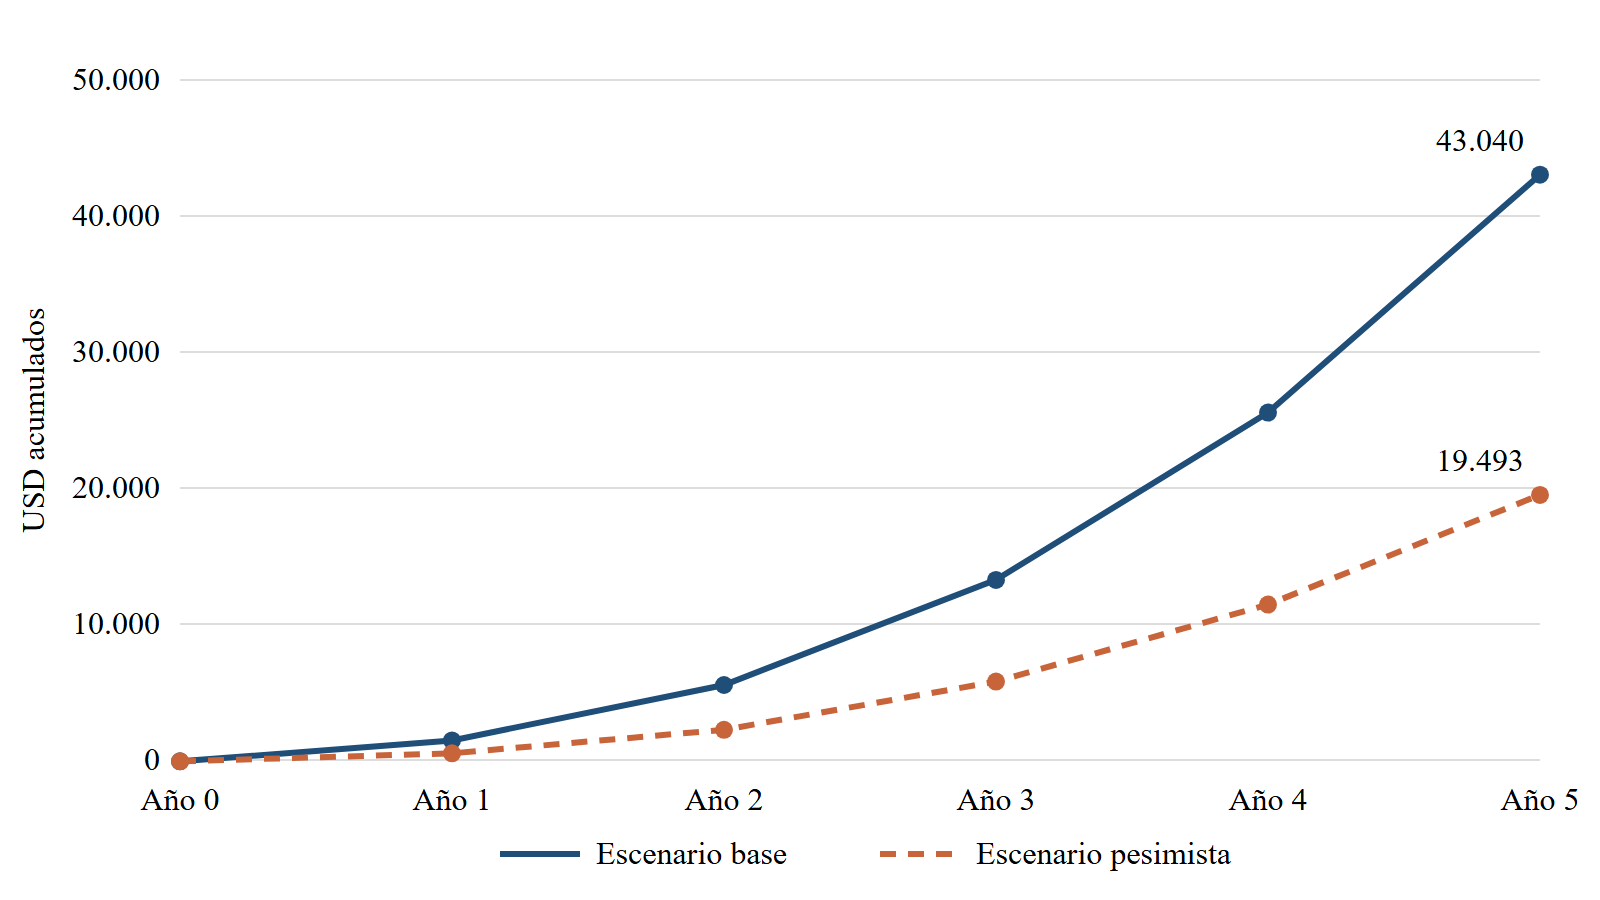
\includegraphics[width=\textwidth]{figuras/fig-5-1}
\caption{Evolución estimada del flujo de caja acumulado en el escenario base y en el pesimista}\label{fig:fig-5-1}
\end{figure}

\section{Período de repago descontado}

El período de repago descontado incorpora la tasa del 20~\% para evaluar en qué momento se recupera la inversión medida en valor presente. El flujo descontado del primer año se ubica en USD 1.284, suficiente para absorber el desembolso inicial de USD 100 dentro de esos mismos doce meses. La fracción requerida (100/1.284) es de 0,08 años, alrededor de 0,9 meses de operación.

\section{Tasa de descuento}

La tasa de descuento se construyó con el modelo de valoración de activos de capital ajustado por riesgo país, sumando una prima por la etapa temprana del proyecto:

\[
r = r_f + \beta \cdot \mathit{PRM} + \mathit{RP} + \text{prima por etapa temprana}
\]

\begin{table}[H]
\centering
\caption{Construcción de la tasa de descuento}\label{tab:c5-tasa}
\small
\begin{tabularx}{\textwidth}{>{\raggedright\arraybackslash}X r >{\raggedright\arraybackslash}X}
\toprule
\tb{Componente} & \tb{Valor} & \tb{Fuente} \\
\midrule
Tasa libre de riesgo $r_f$ (bono del Tesoro de Estados Unidos a 10 años, 15/10/2026) & 5,10~\% & \citet{fred2026} \\
Beta desapalancada del sector software, sistemas y aplicaciones, corregida por caja ($\beta$) & 1,25 & \citet{damodaran2026betas} \\
Prima de riesgo de mercado implícita, enero de 2026 ($\mathit{PRM}$) & 4,23~\% & \citet{bvr2026erp} \\
Riesgo país de Argentina, 23/10/2026 ($\mathit{RP}$) & 7,07~\% & \citet{rava2026} \\
\midrule
Costo del capital propio ($5{,}10 + 1{,}25 \times 4{,}23 + 7{,}07$) & 17,46~\% & Cálculo propio \\
Prima por etapa temprana e iliquidez & 2,54~\% & Estimación propia \\
\textbf{Tasa de descuento adoptada} & \textbf{20,00~\%} & \\
\bottomrule
\end{tabularx}
\end{table}

El proyecto no tiene deuda, por lo que la tasa coincide con el costo del capital propio. La prima por etapa temprana refleja que se trata de un proyecto sin historia de ingresos y sin un mercado secundario para su participación. Es una estimación propia y se fijó para que la tasa total quede en un valor redondo del 20~\%. El riesgo país se tomó en un momento de suba durante octubre de 2026, por lo que la tasa resulta prudente. Si el proyecto avanza hacia una etapa comercial, la tasa deberá recalcularse con los valores vigentes.

\section{Valor Actual Neto (VAN)}

Al descontar los flujos futuros con la tasa de corte del 20~\% anual y restar la inversión inicial, el VAN alcanza un resultado aproximado de USD 21.449. Al arrojar un indicador claramente superior a cero, la propuesta resulta económicamente aceptable bajo los supuestos del escenario base.

\section{Tasa Interna de Retorno (TIR)}

La Tasa Interna de Retorno (TIR) es el porcentaje de descuento que iguala el VAN a cero. Sobre el flujo proyectado, el cálculo arroja una TIR cercana al 1.694~\% anual. Este valor tan elevado no responde a un margen de ganancias desmedido, sino a que la inversión inicial considerada es muy baja en comparación con los flujos netos que se generan desde el primer año.

Por esta razón, la TIR debe interpretarse con cautela y no tomarse de forma aislada. Si bien supera ampliamente la tasa de corte del 20~\%, depende de forma directa de que se cumplan las hipótesis de adopción de los planes pagos.

\section{Punto de equilibrio}

Durante el primer año, los costos operativos fijos (sin contar las comisiones) alcanzan USD 300. Cada suscripción al plan Intermedio aporta, descontada la comisión, unos USD 55,80 al año, y cada suscripción Plus unos USD 167,40. Por lo tanto, el punto de equilibrio operativo se alcanza con seis suscripciones Intermedio, con dos suscripciones Plus o con una combinación de ambas, por ejemplo, una institución y tres familias.

Este cálculo se enfoca en la sostenibilidad operativa y no incluye la amortización del desembolso inicial, que se evalúa con los indicadores de período de repago.

\section{Análisis de escenarios}

El escenario base asume una cantidad creciente de suscripciones a los planes Intermedio y Plus en los años 1 a 5. Para evaluar si el proyecto conserva su viabilidad con una adopción mucho más lenta, se construye un escenario pesimista que reduce aproximadamente a la mitad las suscripciones pagas, manteniendo los precios y los costos fijos.

\begin{table}[H]
\centering
\caption{Escenario pesimista}\label{tab:c5-10}
\footnotesize
\begin{tabularx}{\textwidth}{>{\raggedright\arraybackslash}X l l l l l l}
\toprule
\tb{Concepto} & \tb{Año 0} & \tb{Año 1} & \tb{Año 2} & \tb{Año 3} & \tb{Año 4} & \tb{Año 5} \\
\midrule
Suscripciones (Intermedio / Plus) & 0 & 7 / 3 & 17 / 7 & 32 / 14 & 50 / 22 & 70 / 32 \\
Ingresos & USD 0 & USD 960 & USD 2.280 & USD 4.440 & USD 6.960 & USD 9.960 \\
Costos operativos & USD 0 & USD 367 & USD 550 & USD 896 & USD 1.297 & USD 1.897 \\
Flujo neto & -USD 100 & USD 593 & USD 1.730 & USD 3.544 & USD 5.663 & USD 8.063 \\
Flujo acumulado & -USD 100 & USD 493 & USD 2.223 & USD 5.767 & USD 11.430 & USD 19.493 \\
\bottomrule
\end{tabularx}
\end{table}

En el escenario pesimista, el VAN arroja un valor aproximado de USD 9.618, alrededor de un 55~\% menor que el del escenario base, pero igualmente positivo. La TIR resultante es de aproximadamente 755~\%, y el período de repago se extiende a 0,17 años (2,0 meses) en términos simples y a 0,20 años (2,4 meses) en términos descontados.

Este resultado indica que el proyecto mantiene su viabilidad económica incluso si la adopción resulta la mitad de lo proyectado. El indicador más sensible es el VAN, aunque en ambos escenarios la inversión inicial se recupera dentro del primer año.

El escenario optimista supone un 50~\% más de suscripciones que el escenario base en cada año, con los mismos precios y costos fijos. Mantener los costos fijos es un supuesto favorable, porque una mayor cantidad de usuarios podría requerir más infraestructura.

\begin{table}[H]
\centering
\caption{Escenario optimista}\label{tab:c5-optimista}
\footnotesize
\begin{tabularx}{\textwidth}{>{\raggedright\arraybackslash}X l l l l l l}
\toprule
\tb{Concepto} & \tb{Año 0} & \tb{Año 1} & \tb{Año 2} & \tb{Año 3} & \tb{Año 4} & \tb{Año 5} \\
\midrule
Suscripciones (Intermedio / Plus) & 0 & 23 / 9 & 53 / 23 & 98 / 42 & 150 / 68 & 210 / 98 \\
Ingresos & USD 0 & USD 3.000 & USD 7.320 & USD 13.440 & USD 21.240 & USD 30.240 \\
Costos operativos & USD 0 & USD 510 & USD 902 & USD 1.526 & USD 2.297 & USD 3.317 \\
Flujo neto & -USD 100 & USD 2.490 & USD 6.418 & USD 11.914 & USD 18.943 & USD 26.923 \\
Flujo acumulado & -USD 100 & USD 2.390 & USD 8.808 & USD 20.722 & USD 39.665 & USD 66.588 \\
\bottomrule
\end{tabularx}
\end{table}

La tabla~\ref{tab:c5-escenarios} resume los indicadores de los tres escenarios, primero con la inversión monetaria de USD 100 y después con la inversión valorizada de USD 5.630.

\begin{table}[H]
\centering
\caption{Indicadores de los tres escenarios}\label{tab:c5-escenarios}
\small
\begin{tabularx}{\textwidth}{l R R R R}
\toprule
 & \multicolumn{1}{r}{\tb{Inversión USD 100}} & \multicolumn{3}{c}{\tb{Inversión valorizada USD 5.630}} \\
\cmidrule(lr){2-2}\cmidrule(lr){3-5}
\tb{Escenario} & \tb{VAN} & \tb{VAN} & \tb{TIR} & \tb{Repago descontado} \\
\midrule
Pesimista & USD 9.618 & USD 4.088 & 40~\% & 3,7 años \\
Base & USD 21.449 & USD 15.919 & 79~\% & 2,3 años \\
Optimista & USD 33.282 & USD 27.752 & 109~\% & 1,8 años \\
\bottomrule
\end{tabularx}
\end{table}

Con la inversión valorizada, el VAN sigue siendo positivo en los tres escenarios y la TIR supera la tasa de corte del 20~\% en todos los casos. En el escenario pesimista la inversión se recupera recién en el cuarto año, por lo que la viabilidad depende de que la adopción no caiga por debajo de ese nivel.

\section{Alternativas consideradas}

Se evaluaron distintas alternativas de monetización. La primera versión de este análisis se basaba solo en alianzas institucionales, lo que dejaba la sostenibilidad del proyecto atada a convencer a instituciones y no reconocía que hay familias que sí obtienen un valor concreto, como coordinar a un cuidador contratado y ver lo que registra sin estar presentes.

Una versión intermedia combinaba planes para familias con un abono aparte para instituciones. Se descartó porque obligaba a tener dos tipos de cuenta distintos, cuando una residencia funciona igual que una familia grande, un dueño con varias personas a cargo y varios cuidadores.

También se analizó un modelo basado exclusivamente en publicidad. Aunque habría permitido mantener la gratuidad, su viabilidad exigía un volumen masivo de tráfico y la inclusión de anuncios corría el riesgo de saturar la interfaz en un entorno que requiere máxima claridad.

Finalmente se optó por un modelo de suscripción en tres niveles, con un plan gratuito y dos pagos. Este esquema mantiene gratis lo esencial del día a día, incluida la emergencia, cobra a quienes necesitan coordinar a más personas y sirve igual para una familia que para una institución.

\section{Análisis de impacto}

\subsection{Impacto social}

El principal impacto que busca generar la plataforma es facilitar y centralizar el acceso a la información para quienes tienen a su cargo el cuidado de personas con discapacidad. A través de la organización de los recursos disponibles, el sistema apunta a reducir la dispersión de datos, simplificar la búsqueda de soluciones y brindar recomendaciones personalizadas según las necesidades concretas de cada perfil. Al mismo tiempo, permite que el cuidado se reparta entre varias personas sin perder información, y que las familias sepan cómo se cuida a su familiar, aunque no estén presentes.

\subsection{Impacto institucional}

Para las clínicas, residencias y centros de día, la plataforma ofrece un registro ordenado del cuidado de cada paciente y una herramienta para supervisar a su personal, por ejemplo, detectando tomas de medicación que no se registraron o que se registraron tarde. Además, les permite sumar a las familias de sus pacientes como observadoras, lo que hace más transparente y fluida la comunicación con ellas.

\subsection{Impacto legal}

De cara a una implementación real, será imprescindible considerar de manera rigurosa el marco normativo aplicable a la protección de datos personales, prestando especial atención al tratamiento de información sensible vinculada con personas con discapacidad. Esto incluye definir con claridad quién puede ver la información de cada persona, qué pasa cuando un cuidador deja de trabajar con una familia y cómo se informa el uso de los datos en las instituciones. Asimismo, la plataforma funciona estrictamente como una herramienta de orientación y organización, por lo que no reemplaza en ninguna circunstancia la atención médica ni está facultada para realizar diagnósticos ni emitir prescripciones.

\subsection{Impacto ambiental}

Al tratarse de una solución 100~\% digital, la plataforma no demanda infraestructura física dedicada ni despliegues territoriales para que los usuarios puedan utilizarla. Por este motivo, el impacto ambiental directo de la propuesta es reducido. En una implementación a mayor escala, se deberá considerar la huella de carbono derivada del consumo energético del procesamiento de datos y del alojamiento continuo en servicios cloud.

\section{Supuestos y restricciones}

\begin{itemize}
    \item Los precios de los planes se mantienen constantes en dólares durante los cinco años.
    \item Las comisiones de cobro representan el 7~\% de lo facturado, como supuesto de trabajo.
    \item Los costos de infraestructura, dominio y servicios externos son reservas presupuestarias para una escala pequeña, no cotizaciones firmes.
    \item La cantidad de suscripciones de cada escenario es una estimación propia que no fue validada con familias ni con instituciones.
    \item El valor hora usado para valorizar la inversión es una estimación propia para un perfil junior.
    \item No se consideran impuestos ni la amortización de equipos informáticos.
    \item El proyecto no toma deuda, se financia con el aporte inicial y con los ingresos de las suscripciones.
\end{itemize}

\section{Conclusión}

El análisis económico demuestra la factibilidad del proyecto bajo las condiciones del escenario base definido. La inversión monetaria inicial resulta reducida debido al marco académico en el que se gesta la propuesta y al aprovechamiento de herramientas y servicios de bajo costo o sin cargo. A medida que la plataforma incremente su escala, los costos operativos crecen de forma gradual, mientras que los ingresos se sustentan en las suscripciones de las familias y las instituciones que necesitan más que lo básico.

Los indicadores financieros reflejan un panorama favorable en los tres escenarios, incluso en el pesimista, con la mitad de la adopción prevista, y también cuando se valorizan las horas de trabajo como inversión inicial. No obstante, esto depende de que se cumplan las hipótesis de adopción planteadas, que deberán validarse con usuarios e instituciones reales antes de una implementación comercial.

